\graphicspath{{./figures/}}


In this section, we provide a brief history of neural networks in the context of finance and time series prediction, as well as a more detailed description of the architecture used in the paper.

Neural networks are systems largely belonging to the study of Machine Learning, typically associated with solving computational problems that other models and algorithms struggle to. Loosely based on biological neural networks, like the brain, artificial neural networks are collections of neuron-like nodes and links that connect them. Their resemblance to the brain in terms of architecture is part of what allowed neural networks to grow in computing power and popularity over the past decades, from their emergence in the 1940s.\citesuper{nervenets}\citesuper{nervous_activity_warrenpitts}

\section{Neurons}
Neurons are the artificial equivalent of a biological neuron and are the fundamental components of a neural network. Neurons perform three tasks, receive input from other neurons, apply an activation function to the input and output a value to other neurons. Neurons in the network are connected and each of these connections carries a signal and has certain weight attached to it, which affects the signal carried.\citesuper{machine-learning-dict}\citesuper{ai_book} Graphically, a neuron could be represented in figure \ref{tab:neuron}.

\begin{figure}[h]
    \centering
    \begin{tikzpicture}[
        init/.style={
        draw,
        circle,
        inner sep=2pt,
        font=\Huge,
        join = by -latex
        },
        squa/.style={
        draw,
        inner sep=2pt,
        font=\Large,
        join = by -latex
        },
        start chain=2,node distance=13mm
        ]
        \node[on chain=2] 
        (x2) {$x_2$};
        \node[on chain=2,join=by o-latex] 
        {$w_2$};
        \node[on chain=2,init] (sigma) 
        {$\displaystyle\Sigma$};
        \node[on chain=2,squa,label=above:{\parbox{2cm}{\centering Activation \\ function}}]   
        {$f$};
        \node[on chain=2,label=above:Output,join=by -latex] 
        {$y$};
        \begin{scope}[start chain=1]
        \node[on chain=1] at (0,1.5cm) 
        (x1) {$x_1$};
        \node[on chain=1,join=by o-latex] 
        (w1) {$w_1$};
        \end{scope}
        \begin{scope}[start chain=3]
        \node[on chain=3] at (0,-1.5cm) 
        (x3) {$x_3$};
        \node[on chain=3,label=below:Weights,join=by o-latex] 
        (w3) {$w_3$};
        \end{scope}
        \node[label=above:\parbox{2cm}{\centering Bias \\ $b$}] at (sigma|-w1) (b) {};
        
        \draw[-latex] (w1) -- (sigma);
        \draw[-latex] (w3) -- (sigma);
        \draw[o-latex] (b) -- (sigma);
        
        \draw[decorate,decoration={brace,mirror}] (x1.north west) -- node[left=10pt] {Inputs} (x3.south west);
    \end{tikzpicture}
    \caption{Graphical representation of a Neuron}
    \label{tab:neuron}
\end{figure}

\section{Activation Functions}
\citeauthor{machine-learning-dict} (\citeyear{machine-learning-dict}) defines the activation function of a neural network as the function that governs the output behaviour of a neuron, given a set of input values. There are several types of activation functions, the simplest being the step function.

In mathematical terms, the step function, or the unit step function, is defined as

\begin{align}
    \centering
    H(x) := \begin{cases}
        0, & \text{for } x < 0 \\
        1, & \text{for } x \geq 0
    \end{cases}
\end{align}

where $H(x)$ is the Heaviside step function\citesuper{step_function}. At value 0, an output of $H(0) = 1$ is selected and passed down to the next layer of neurons.

\subsection{Rectified Linear Unit}
The Rectified Linear Unit (ReLU) is an activation function mathematically defined as 

\begin{align}
    \centering
    f(x) = [x]^+ = \text{max}(0, x) 
\end{align}

where $x$ is the neuron's input value. Plotted on cartesian axes, the graph shows a linear relationship for $f(x)$ and $x$ where $x > 0$. Generating a plot of ReLU further explains its activation range.

\begin{figure}[H]
    \centering
    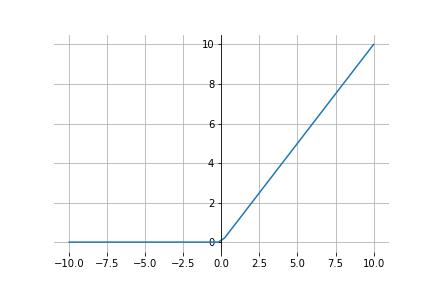
\includegraphics[width=85mm]{relu}
    \caption{Plot of the Rectified Linear Unit function}
    \label{tab:relu}
\end{figure}

ReLU was first introduced in the 2000 and 2001 Hahnloser papers.\citesuper{relu2000}\citesuper{relu} ReLU is currently the most widely used activation function\citesuper{acti-functions} and has found great success in training deep neural networks primarily in the fields of computer vision\citesuper{relu-vision} and speech recognition.\citesuper{relu-acoustics}

\subsection{Sigmoid}
The Sigmoid function is a logistic activation function, mathematically defined as 

\begin{align}
    \centering
    f(x) = \frac{L}{1 + e^{-k(x-x_0)}}
\end{align}

where 
\begin{itemize}[nosep]
    \item[] $L$ is the maximum point of the curve,
    \item[] $k$ is the steepness of the curve,
    \item[] $x_0$ is the value of the midpoint of the curve. 
\end{itemize}

Sigmoid functions are non-linear, differentiable, defined for all real input values and have an output greater than zero for all inputs, in contrast to the ReLU activation function whose output is greater than zero only with positive inputs. A well known example of a sigmoidal curve is the cumulative distribution function of the normal distribution.

\begin{figure}[H]
    \centering
    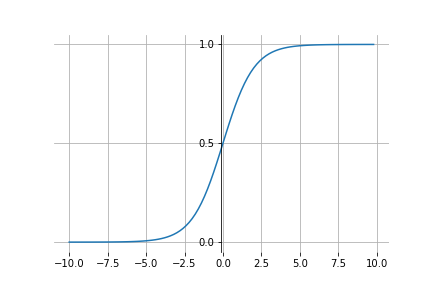
\includegraphics[width=85mm]{sigmoid}
    \caption{Plot of the sigmoid function}
    \label{tab:sigmoid}
\end{figure}

\subsection{Hyperbolic tangent}
The hyperbolic tangent is a specialised case of the sigmoid function, mathematically defined as 

\begin{align}
    f(x) = \text{tanh}(x) = \frac{e^{2x} - 1}{e^{2x} + 1}
\end{align}

Unlike the standard sigmoid function, tanh can output negative values for negative inputs giving it double the range that the standard sigmoid has.

\begin{figure}[H]
    \centering
    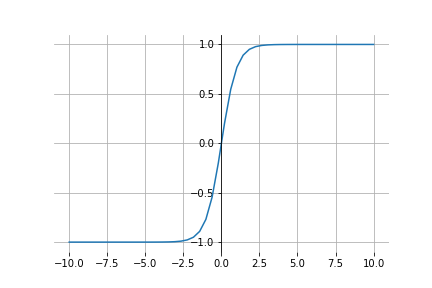
\includegraphics[width=85mm]{tanh}
    \caption{Plot of the hyperbolic tangent function}
    \label{tab:tanh}
\end{figure}

\section{Backpropagation}
The backpropagation algorithm is a key feature of neural networks as it allowed for fast and efficient training of multi-layered networks by distributing error values back through the layers of the network, adjusting the weights in the connections between neurons respectively.\citesuper{backprop} In more detail, backpropagation functions compute the gradient $\nabla_{x}f(\mathbf{X}, \mathbf{y})$ numerically in a simple and inexpensive procedure.\citesuper{rumelhart_backprop} What computing the gradient really means is calculating the derivative of the loss function in the model, with the loss function being a selected error function, a historically popular function being the sigmoid function described in the previous section.

\newcommand{\R}{\mathbb{R}}

The chain rule is a way to calculate the derivate of functions by decomposing a function to other functions whose derivative is known. Let $x$ be a real number and $f$ and $g$ be functions that map from $\R$ to $\R$. By generalising the chain rule of calculus
\begin{align}
    \frac{dz}{dx} &= \frac{dz}{dy}\frac{dy}{dx}
\end{align}
one could compute the partial derivatives of the error at node $ (i, j)$ with weight $w$ 
\begin{align}
    \frac{\partial z}{\partial x_i} &= \sum\limits_{j} \frac{\partial z}{\partial y_j}\frac{\partial y_j}{\partial x_i}
\end{align}
Computing all these derivatives and putting them in a matrix of size $n\times m$ where $n = i$ and $m = j$ constructs the Jacobian matrix for the function $z = f(x)$. A Jacobian matrix is formally defined as the matrix of all first-order partial derivatives of a vector-valued function.
\begin{figure}[H]
    \centering
    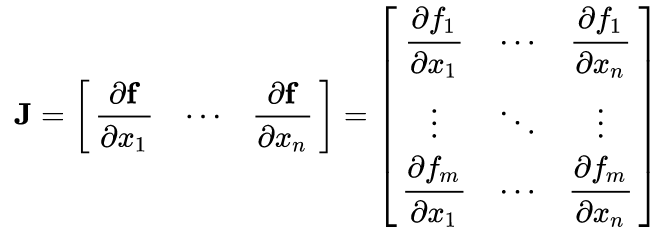
\includegraphics[scale=0.6]{jacobian.png}
    \label{tab:jacobian}
    \caption{Matrix representation of the Jacobian matrix\citesuper{jacobian_img} $\mathbf{J}$ of function $\mathbf{f}$. Every entry $(i, j)$ in the matrix is $\mathbf{J}_{i, j} = \frac{\partial f_i}{\partial x_j}$}
\end{figure}
Backpropagation performs this calculation for every single node in the network moving backwards, updating the weights on the nodes as it moves, effectively training the network\citesuper{goodfellow_backprop}. Backpropagation is so efficient, it has become the most popular algorithm in training neural networks, along with the sigmoid being one of the most popular activation functions demonstrated in backprop algorithms due to its easy and simple derivative.

\section{LSTM}
Long Short-Term Memory (LSTM) is a type of recurrent neural network first introduced in \citeyear{lstm} by \citeauthor{lstm}. Like all recurrent networks, LSTM differs from feed-forward networks by incorporating cyclical connections between neurons.

The LSTM was introduced specifically to address the two problems of the \emph{vanishing gradient problem} and the \emph{exploding gradient problem}. The two problems are closely linked problems regarding the propagation of errors in deep neural networks. In short, the two gradient problems appear when attempting to train networks with gradient-based learning, iterative methods for computing the gradient at each sample point, like the backpropagation method described above, and either cause the gradient to be "vanishingly" small (\emph{vanishing gradient}) or to "explosively" increase (\emph{exploding gradient}).\citesuper{vanishing}\citesuper{rnn_vanishing}

\begin{figure}[H]
    \centering
    \begin{subfigure}{.5\textwidth}
        \centering
        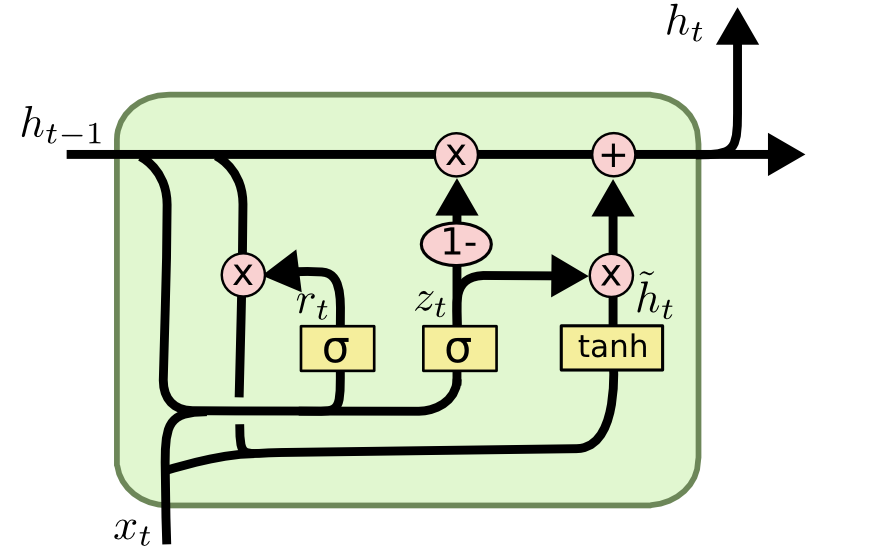
\includegraphics[width=100mm]{lstm_cell.png}
        \label{tab:lstm_cell}
    \end{subfigure}%
    \centering
    \begin{subfigure}{.5\textwidth}
        \centering
        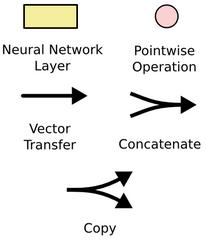
\includegraphics[height=60mm]{lstm_objects_info_matrix.png}
        \label{tab:lstm_cell_info}
    \end{subfigure}
    \caption{Diagram of the LSTM cell}
\end{figure}
